\chapter{Conclusions and future work}
\label{chap:conclusion}

\section{Results, uncertainties and the need of new invariants}

\bigskip \centerline{\bf \textsc{Blink Calculus}} \bigskip
The first contribution of this thesis that we want to stress
here was given in Section~\ref{sec:blinkCalculus}. Based on the BFL
calculus (\ie Kirby's calculus reformulated in BFL language) we obtained
a purely blink calculus. This calculus is a formal language
which is a counterpart for homeomorphism of spaces. \hbox{Figure~\ref{fig:blinkCalculusOnCoins2}}
presents again our blink calculus. Although theoretically complete (it is supported by Kirby's Calculus) this calculus was not
used in our computational experiments as a tool to prove homeomorphisms.
For this task we used the combinatorial simplification dynamics of
3-gems. In spite of that, we think that the blink calculus can help
in the search for new space invariants.

\begin{figure}[htp]
   \begin{center}
      \leavevmode
      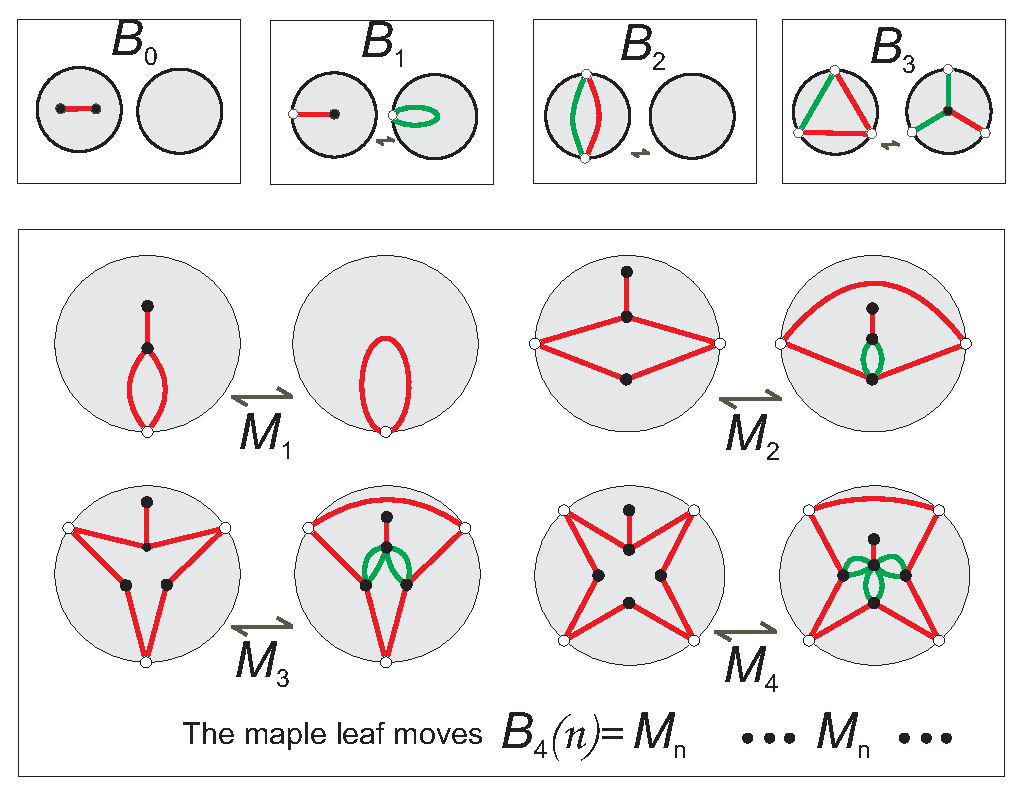
\psfig{file=fig/blinkCalculusOnCoins.eps,width=10cm}
   \end{center}
   \vspace{-0.7cm}
   \caption{Blink formal calculus by local coins replacements}
   \label{fig:blinkCalculusOnCoins2}
\end{figure}

\bigskip \centerline{\bf \textsc{Decomposition/Composition Theory}}
A second contribution of this work that was important to the
computational results are the following propositions and theorems
in g-blink language:

\noindent {{\bf (Theorem on partial dual \ref{theo:partialDual})} \,\, \it
Let $A$ and $B$ be arbitrary disjoint
g-blinks, $(a,b)$ a basepair on them. Then
 $A[a] + B[b] \Sequiv A[a] + \textsc{Dual}(B)[b]$.
}

\noindent {{\bf (Theorem on partial reflection \ref{theo:partialReflection})} \,\, \it
Let $A$ and $B$ be arbitrary disjoint g-blinks, $(a,b)$ a basepair
on them. Then($A[a] + B[b] \Sequiv A[a] +
\textsc{Reflection}(B)[b].$
}


\noindent {{\bf (Theorem on partial refDual \ref{theo:partialRefDual})} \,\, \it
Let $A$ and
$B$ be arbitrary disjoint g-blinks, $(a,b)$ a basepair on them. Then
$A[a] + B[b] \Sequiv A[a] + \textsc{RefDual}(B)[b].$
}

The third theorem on partial refDuals is obtained directly from the framed link theory.
Given this third theorem, the first two theorems are equivalent: given one we have the other.
The theorem on partial reflection was tricky to obtain. We
used both the theory of gems and the \textsc{Blink2Gem} algorithm as well as topological machinery
to exhibit an explicit homeomorphism.
Section~\ref{sec:proofOfThePartialReflectionTheorem} contains
this proof. These theorems yield a block decomposition/composition
theory which leads to the representative concept and curtailed search
spaces of our computational experiments.

\bigskip \centerline{\bf \textsc{An unavoidable set of blinks up to 9 edges}} \bigskip

We achieved our initial main objective which was to classify
spaces presentable by blinks with small number $n$ of edges.
At the level of $n \leq 9$ the combination of tools
\begin{itemize}
\item theory of decomposition/composition leading to representative g-blinks --- which reduces the search space
\item quantum invariants and homology --- which provide distinctiveness
\item combinatorial simplification dynamics of 3-gem theory --- which provides similarity
\end{itemize}
was as effective as leaving only two uncertainties in more than 500 spaces.
These uncertainties, as we saw in Section~\ref{sec:topologicalClassificationOfU}, were registered
as Conjecture\ref{conj:conjecture1}~and~Conjecture~\ref{conj:conjecture2}.
To be honest, these conjectures are actually doubts and
seem an interesting research problem. It could be answered by a new invariant
which complements the HGnQI invariant. In any case (\ie the two
conjectures are false, or one is true and the other is false, or both are true) the
relevant fact is that any space that has a blink presentation with up to 9
edges is induced by only one of the classes in Appendix~\ref{chap:primeCatalogue},
where classes 9.126 and 9.199 may be broken into two classes each. A space
that is not prime and has a blink presentation with $\leq 9$ edges is
just a blink with more than one prime component which is in the catalogue
(Section~\ref{sec:census}).

\begin{figure}[h!tp]
   \begin{center}
      \leavevmode
      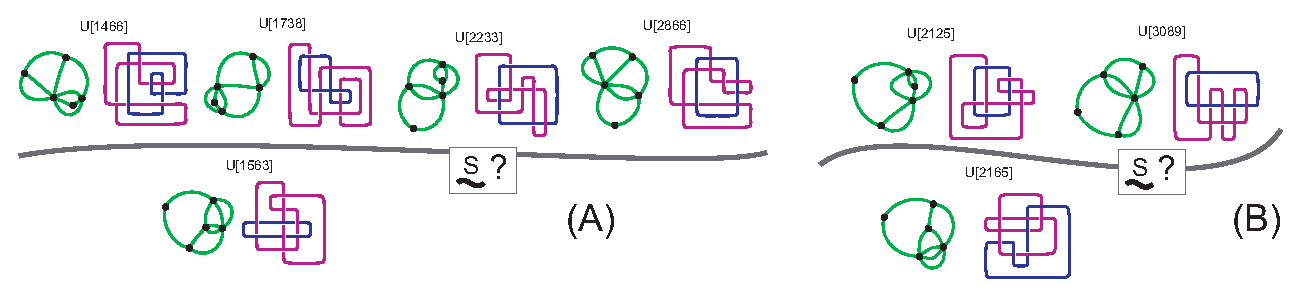
\psfig{file=fig/doubts.eps,width=16cm}
   \end{center}
   \vspace{-0.7cm}
   \caption{ The only 2 classes with same HGnQI where a proof of the homeomorphism was not found}
\end{figure}

In the case of simple 3-connected monochromatic blinks with up to 16
edges there are only the 11 uncertainties shown in Figure~\ref{fig:doubts3ConnectedIsolated2}.
We did not use the simplification combinatorial dynamics of 3-gems
to deal with these cases.

\begin{figure}[h!tp]
   \begin{center}
      \leavevmode
      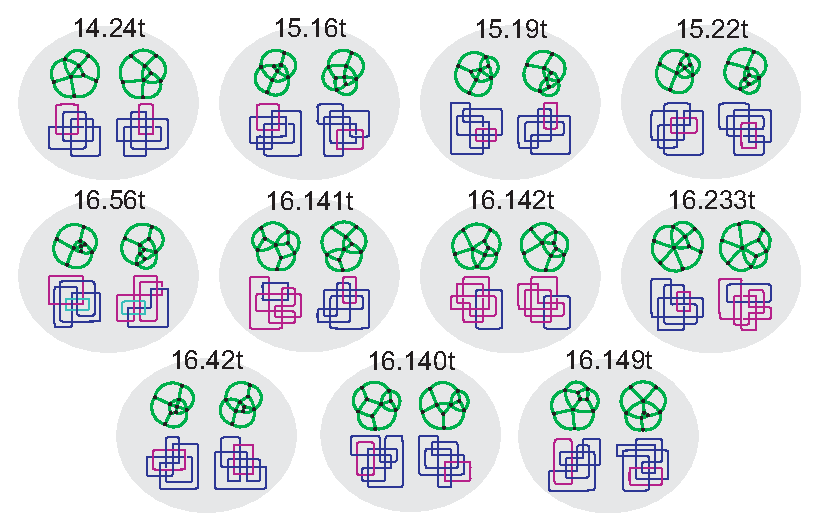
\psfig{file=fig/doubts3ConnectedIsolated.eps}
   \end{center}
   \vspace{-0.7cm}
   \caption{ Doubts on simple 3-connected all green blinks}
   \label{fig:doubts3ConnectedIsolated2}
\end{figure}

Putting together blinks that induce the same space in a non-trivial
way (Appendix~\ref{chap:primeCatalogue},
Appendix~\ref{chap:compositeCatalogue} and
Appendix~\ref{chap:catalolgue3con}) we hope to
be contributing with non-trivial examples that can
motivate and help the search for new effective
subtle invariants of spaces to complement the
HGnQI invariant.


\newpage

\section{The inverse algorithm: from gem to blink}

A rather frustrating fact up to now is that we could not find a blink
for the space ${\rm EUCLID}_1$. This space is generated by the rigid
gem $r_{5}^{24}$ (notation of 3-gems catalog of \cite{Lins1995}). Blinks
and BFLs for the other euclidean spaces are given below.
\begin{center}
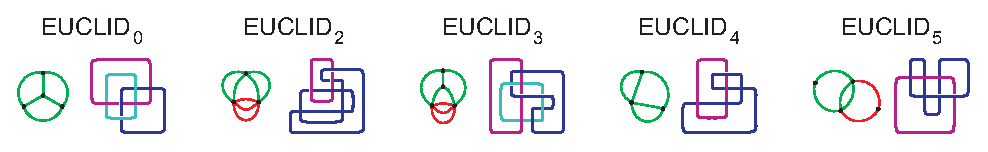
\psfig{file=fig/euclids.eps,width=14cm}
\end{center}
They correspond, respectively, to spaces 6.8, 7.10, 8.32, 5.4 and 6.13. By looking at quantum
invariants of these spaces (see Appendix~\ref{chap:primeCatalogue}) we are
led to the following conjecture.
\begin{conjecture}
The absolute value of the quantum invariants of the euclidean
spaces are non-negative integers for all levels $r$.
\end{conjecture}
The missing ${\rm EUCLID}_1$ space motivates the
following discussion.

There exists a rather simple algorithm to go from a framed link
inducing a space to a triangulation of the same space. This was
first done in chapter 11 of~\cite{KauffmanAndLins1994} via {\em
graph encoded 3-manifolds} or {\em gems}. This algorithm was
improved here in Section~\ref{sec:fromGBlinkTo3Gem} and it is
a central tool in the \textsc{Blink} program to prove spaces
in $U$ are homeomorphic. Figure~\ref{fig:blink2GemAlgorithm}
shows this algorithm. Thus to get a gem from a blackboard
framed link is a direct task.
\begin{figure}[htp]
   \begin{center}
      \leavevmode
      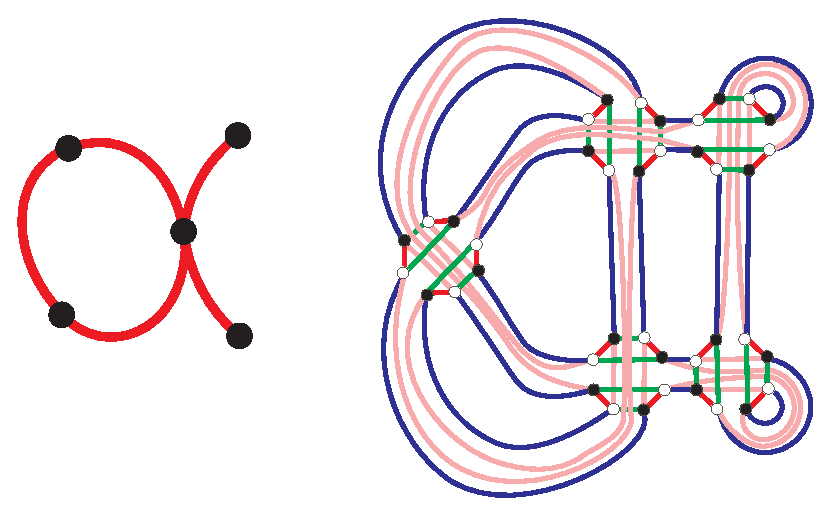
\psfig{file=fig/blink2GemAlgorithm.eps,width=8cm}
   \end{center}
   \vspace{-0.7cm}
   \caption{ Blink to gem algorithm: indispensable to prove homeomorphisms of blinks}
   \label{fig:blink2GemAlgorithm}
\end{figure}

However, the contrary, given a gem to find by
a polynomial algorithm a blackboard framed link inducing the same
3D-space is, as far as we know, an untouched problem in the
literature. Figure~\ref{fig:spacePresentationsSchema} shows this computational gap as a red arrow.
The reason why it is desirable to have this arrow in black
stems from the fact that the quantum invariants are not computable
from a triangulation or gem based presentation of 3D-spaces. The two
languages, triangulations and blackboard framed links have at
present only a one way translation.

\begin{figure}[htp]
   \begin{center}
      \leavevmode
      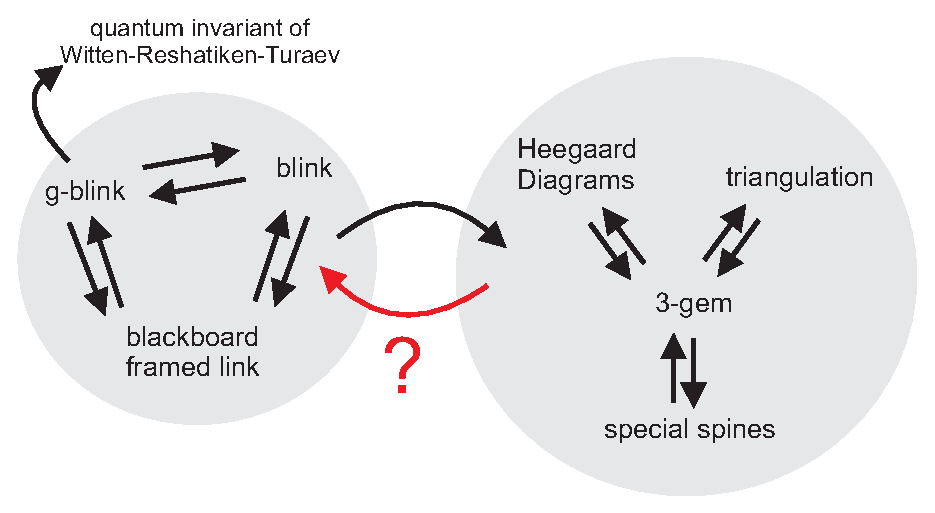
\psfig{file=fig/spacePresentationsSchema.eps,width=8cm}
   \end{center}
   \vspace{-0.7cm}
   \caption{ Blink based presentation and 3-Gem based presentation}
   \label{fig:spacePresentationsSchema}
\end{figure}

Trying to get this converse algorithm took a long a time of our research for this thesis.
Only recently we got confident that we have succeeded. A first step in this direction was given
in the paper~\cite{Lins2007}, where a linear algorithm to prove the
Lickorish-Wallace Theorem is provided. The second part, which actually
presents the blink from the gem
is a joint work with S. Lins \cite{LinsLins2007} and
awaits a proper computer implementation. The first test of
this implementation will be to get a blink for ${\rm EUCLID}_1$.

\section{The \textsc{Blink} computer program}

A computer program to manipulate spaces through its many
possible presentations was one of our goals in this work.
Indeed, a great effort was made to bring \textsc{Blink}
to life: a program written in Java that, at this moment,
has more than 800 hundred classes and more than 70000
lines of code. Today, \textsc{Blink} supports
blinks, g-blink, BFLs and 3-gems. The idea is, in
the future, to bring other possible space presentations,
like special spines, into it.

To make \textsc{Blink} a flexible program we decided that its
interface would be a {\it Command Line Interface}. It displays
a prompt and the user enters a command or a script written in
a {\it language} that we also name \textsc{Blink}. Once a
command or script has been entered, the program calculates
the script result and shows it to the user. The flexibility we
get in this type of design is good; for example we can
combine functions and easily express more complex functions.

Besides the calculation of invariants, the identification of certain
structures into 3-gems (\eg disconnecting quartets, dipoles) or
into g-blinks (\eg simplification points) one of the main characteristics of
\textsc{Blink} is its capability of presenting drawings or
diagrams for blinks, g-blink, BFLs and 3-gems. Almost all
drawings on this thesis came from \textsc{Blink}. To get
good looking and correct drawings for blinks,
g-blinks and BFLs took us a long time once we didn't
know a good way of doing it. But finally we found a
great solution: {\em Tamassia's Algorithm \cite{Tamassia1987}}.

We have implemented the following four algorithms to
deal with the drawing issue. Except for the first algorithm,
the other three are further fine-tuned with {\em B�zier curves and
splines techniques} (\cite{FoDaFeHu1990}) to produce
rounded-drawings with curved edges.

\begin{enumerate}
\item {\em Coin-drawing Algorithm:} this was our own first original
algorithm which we implemented to correctly draw in a visible scale
the whole of any plane graph. The drawing is in the interior of a
disk named a {\em coin}. The coin-drawing algorithm chooses and draw
a spanning tree of the graph with appropriate lengths and angles.
These ensure that the remaining edges can be displayed as a path
which is a line segment, an arc of circle and another line segment.
This is the simplest algorithm producing the less pleasing
aesthetical effect. Nevertheless, these {\em coin-drawings} are
important because they were, for a long time in our work, the only
general method with total visibility. Figure~\ref{fig:coinDrawing} presents
an example of our coin drawing algorithm.

\begin{figure}[htp]
   \begin{center}
      \leavevmode
      
\psfig{file=fig/coinDrawing.eps}
   \end{center}
   \vspace{-0.7cm}
   \caption{ Coin drawing of $U[1078]$}
   \label{fig:coinDrawing}
\end{figure}

\item {\em Tutte's Barycentric Algorithm \cite{Tut1967}:}
we have implemented this well known algorithm that draws a
$3$-connected plane graph by choosing the external face and
extending the drawing so that every interior vertex is in the
barycenter of its neighbors. Frequently, it produces pleasant
drawings. However it does not treat the less connected graphs which
are central for our work: loops, pendant vertices and cut-vertices
are of fundamental importance in blink theory. Another problem that
occurs with Tutte's based algorithm is the one of discrepant scales:
some parts of the drawing are exponentially smaller that others, and
simply disappear from the drawings. Despite of these
disadvantages, Tutte's algorithm works well for the majority of
blinks in the set $U$.

\item {\em Koebe, Andreev
and Thurston's Theorem on circle packing in the hyperbolic plane:}
beautiful drawings of plane graphs are possible to obtain from the
geometry of the hyperbolic plane. Given a $3$-connected plane graph,
there exist circles centered at the vertices of the graph so that
the edges are defined by the contact points of two circles. See the
articles of Smith~\cite{Smith1994}, Stephenson~\cite{Ste2003} of
Collins and Stephenson~\cite{CoSte2003} where algorithms are
outlined for the case of triangulations.  The Theorem yielding the
circle packing was proved independently by Koebe \cite{Koebe1936},
Andreev \cite{Andreev1970} and by Thurston \cite{Thurston1982}.
We have implemented our own version of the algorithm which works in
the case of $3$-connected graphs. However, it suffers the same
disadvantages as Tutte's Algorithm. Nevertheless, when it works it
produces the nicest results. Figure~\ref{fig:circlePacking} presents a
blink, its BFL, the circle packing that defined the first two drawings,
and the first three drawings together.

\begin{figure}[h!tp]
   \begin{center}
      \leavevmode
      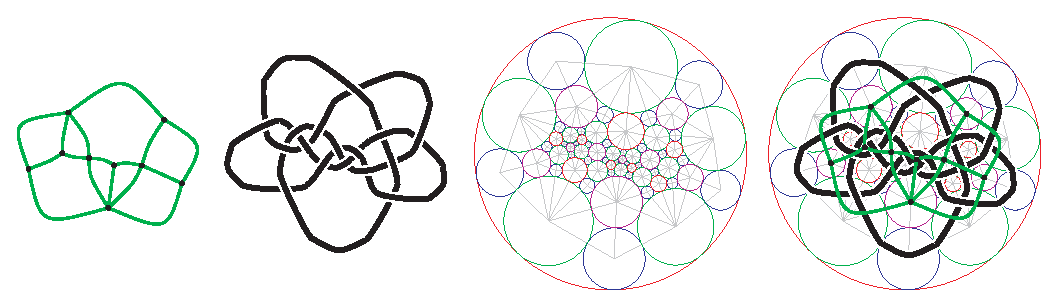
\psfig{file=fig/circlePacking.eps,width=14cm}
   \end{center}
   \vspace{-0.7cm}
   \caption{ Circle packing of a 3-connected blink}
   \label{fig:circlePacking}
\end{figure}

\item {\em Tamassia's Algorithm \cite{Tamassia1987}: to embed an arbitrary
plane graph with valency at most 4 in the rectilinear grid so as to
minimize the number of bends.} This algorithm came to our attention
only at latter phase of our research. Fine-tunings of it has all the
properties we needed: it correctly draws any plane graph and it does
not suffer from the undesirable phenomenon of discrepant scales:
all the vertices and the edges are entirely well visible. The
objective of the method is to minimize (in a precisely defined
mathematical way) the number of bends. The algorithm depends three
times on the algorithm to compute a minimum cost-flow in a network.
The essence of this algorithm is in the design of the first network.
Each feasible flow in this network encodes valid ``shapes'' for the edges 
of the graph. This encoding tells, for example, that an edge has no 
bends or that it has one bend to the right then one bend to the left.
When a minimum flow is found in this network the minimum number of 
bends for a valid rectilinear embedding of the given graph is found. The 
other two networks are used to find the lengths of the horizontal
end vertical segments of the edges. In order to have Tamassia's 
algorithm available, we had first to implement the minimum cost flow 
algorithm in its full generality via the network simplex method. We 
have based our implementation on the lucid exposition Chapter 19 
of \cite{Chvatal1983} and in the
(editor's categorization) ``Exceptional Paper'' \cite{BrBrGr1977},
which is the original source of the network simplex method.
Tamassia's algorithm is an unexpected application of network flow
theory in its full strength. Since its publication in 1987, it has
become a theoretically beautiful at the same time a practical
device used on dozens of applications. Having implemented it from
scratch, we had the opportunity of tailoring it to fulfill our
expectations on drawing of general plane graphs. In particular, the
restriction about the maximum degree 4 is easy to overcome. Finally,
the use of B�zier curves and splines (\cite{FoDaFeHu1990}) makes the
drawings more pleasing aesthetically, with smaller perceptual
complexity. All drawings in the Appendices are based in this algorithm.
\end{enumerate} \enlargethispage{1cm}

We want to make \textsc{Blink} an open source project on the
internet but this wasn't done yet.

\newpage

\centerline{\bf \textsc{An example of Blink usage}} \bigskip

We finish this section with an example of the usage of
\textsc{Blink}. Here is the code:

\begin{center}
\begin{minipage}{14cm}
\begin{footnotesize}
\setstretch{1.1}
\begin{verbatim}
// associates B to the g-blink with 4 parallel green edges: U[5]
B = gblink(5)
// all possible toroidal sums with B up to 24 edges
C = combineGBlinks({B},24)
// calculate representative
C = rep(C)
// remove duplicates
C = set(C)
// homology groups on all g-blink of C
HGs = hg(C)
// calculate quantum invariant on all g-blink of C up to level 4
QIs = qi(C,4)
// produces the blink drawings
db(C,cols=10,rows=4,eps="blinks.eps")
// produces the link drawings
dl(C,cols=10,rows=4,eps="links.eps")
\end{verbatim}
\end{footnotesize}
\end{minipage}
\end{center}

The BFL presentation of $U[5]$ is the first in $U$
to have two components. It is a blink with four parallel
green edges. By merging $U[5]$ with itself in all possible
ways we obtain 38 representative blinks with $\leq$
24 edges. These 38 blinks and their associated
BFLs are shown in Figure~\ref{fig:blinkLanguageExample}.
We calculated homology group and  the quantum invariant
up to level 4 of these 38 blinks. We could distinguish
24 spaces. The blinks we cannot distinguish with this
experiment are:
$\{ 9, 12\}$,
$\{10, 13\}$,
$\{16, 27, 36\}$,
$\{17, 19, 25, 28\}$,
$\{18, 21, 26, 29, 31\}$,
$\{20, 24\}$,
$\{23, 30\}$,
$\{32, 34\}$.

\def\rsep{0cm}%-0.15cm}

\begin{center}
\begin{scriptsize}
\begin{tabular}{cccc}
\# & HG & r=3 & r=4 \\[\rsep]
01 & $2^2    $ & $1.41421 + 0.00000i$ & $ 1.50000 -  0.50000i$ \\[\rsep]
02 & $(1)\, 2^2$ & $2.00000 + 0.00000i$ & $ 2.00000 -  1.00000i$ \\[\rsep]
03 & $2^4    $ & $2.82842 + 0.00000i$ & $ 3.00000 -  2.00000i$ \\[\rsep]
04 & $(2)\, 2^2$ & $2.82842 + 0.00000i$ & $ 3.00000 -  1.00000i$ \\[\rsep]
05 & $(1)\, 2^4$ & $4.00000 + 0.00000i$ & $ 5.00000 -  3.00000i$ \\[\rsep]
06 & $(1)\, 2^4$ & $4.00000 + 0.00000i$ & $ 4.00000 -  4.00000i$ \\[\rsep]
07 & $(3)\, 2^2$ & $4.00000 + 0.00000i$ & $ 6.00000 +  0.00000i$ \\[\rsep]
08 & $(2)\, 2^4$ & $5.65685 + 0.00000i$ & $ 8.00000 -  6.00000i$ \\[\rsep]
09 & $2^6    $ & $5.65685 + 0.00000i$ & $ 7.00000 -  7.00000i$ \\[\rsep]
10 & $(2)\, 2^4$ & $5.65685 + 0.00000i$ & $ 6.00000 -  6.00000i$ \\[\rsep]
11 & $2^6    $ & $5.65685 + 0.00000i$ & $ 5.00000 -  7.00000i$ \\[\rsep]
12 & $2^6    $ & $5.65685 + 0.00000i$ & $ 7.00000 -  7.00000i$ \\[\rsep]
13 & $(2)\, 2^4$ & $5.65685 + 0.00000i$ & $ 6.00000 -  6.00000i$ \\[\rsep]
14 & $(2)\, 2^4$ & $5.65685 + 0.00000i$ & $10.00000 -  4.00000i$ \\[\rsep]
15 & $(4)\, 2^2$ & $5.65685 + 0.00000i$ & $14.00000 +  2.00000i$ \\[\rsep]
16 & $(1)\, 2^6$ & $8.00000 + 0.00000i$ & $14.00000 - 12.00000i$ \\[\rsep]
17 & $(1)\, 2^6$ & $8.00000 + 0.00000i$ & $ 8.00000 - 12.00000i$ \\[\rsep]
18 & $(1)\, 2^6$ & $8.00000 + 0.00000i$ & $10.00000 - 12.00000i$ \\[\rsep]
19 & $(1)\, 2^6$ & $8.00000 + 0.00000i$ & $ 8.00000 - 12.00000i$ \\[\rsep]
\end{tabular}
\begin{tabular}{cccc}
\# & HG & r=3 & r=4 \\[\rsep]
20 & $(1)\, 2^6$ & $8.00000 + 0.00000i$ & $ 8.00000 - 14.00000i$ \\[\rsep]
21 & $(1)\, 2^6$ & $8.00000 + 0.00000i$ & $10.00000 - 12.00000i$ \\[\rsep]
22 & $(1)\, 2^6$ & $8.00000 + 0.00000i$ & $ 6.00000 - 12.00000i$ \\[\rsep]
23 & $(1)\, 2^6$ & $8.00000 + 0.00000i$ & $ 8.00000 - 10.00000i$ \\[\rsep]
24 & $(1)\, 2^6$ & $8.00000 + 0.00000i$ & $ 8.00000 - 14.00000i$ \\[\rsep]
25 & $(1)\, 2^6$ & $8.00000 + 0.00000i$ & $ 8.00000 - 12.00000i$ \\[\rsep]
26 & $(1)\, 2^6$ & $8.00000 + 0.00000i$ & $10.00000 - 12.00000i$ \\[\rsep]
27 & $(1)\, 2^6$ & $8.00000 + 0.00000i$ & $14.00000 - 12.00000i$ \\[\rsep]
28 & $(1)\, 2^6$ & $8.00000 + 0.00000i$ & $ 8.00000 - 12.00000i$ \\[\rsep]
29 & $(1)\, 2^6$ & $8.00000 + 0.00000i$ & $10.00000 - 12.00000i$ \\[\rsep]
30 & $(1)\, 2^6$ & $8.00000 + 0.00000i$ & $ 8.00000 - 10.00000i$ \\[\rsep]
31 & $(1)\, 2^6$ & $8.00000 + 0.00000i$ & $10.00000 - 12.00000i$ \\[\rsep]
32 & $(3)\, 2^4$ & $8.00000 + 0.00000i$ & $14.00000 - 10.00000i$ \\[\rsep]
33 & $(3)\, 2^4$ & $8.00000 + 0.00000i$ & $12.00000 -  8.00000i$ \\[\rsep]
34 & $(3)\, 2^4$ & $8.00000 + 0.00000i$ & $14.00000 - 10.00000i$ \\[\rsep]
35 & $(3)\, 2^4$ & $8.00000 + 0.00000i$ & $ 8.00000 -  8.00000i$ \\[\rsep]
36 & $(1)\, 2^6$ & $8.00000 + 0.00000i$ & $14.00000 - 12.00000i$ \\[\rsep]
37 & $(3)\, 2^4$ & $8.00000 + 0.00000i$ & $22.00000 -  6.00000i$ \\[\rsep]
38 & $(5)\, 2^2$ & $8.00000 + 0.00000i$ & $32.00000 +  4.00000i$ \\[\rsep]
\end{tabular}
\end{scriptsize}
\end{center}
\enlargethispage{2cm}
Observe the curious fact that, except for the first blink, the quantum
invariants at level $r=4$ are Gauss integers (\ie $a + bi$ with $a,
b$ integers). This type of experiment is very easy to do with \textsc{Blink}.

\newpage

\begin{figure}[h!tp]
   \begin{center}
      \leavevmode
      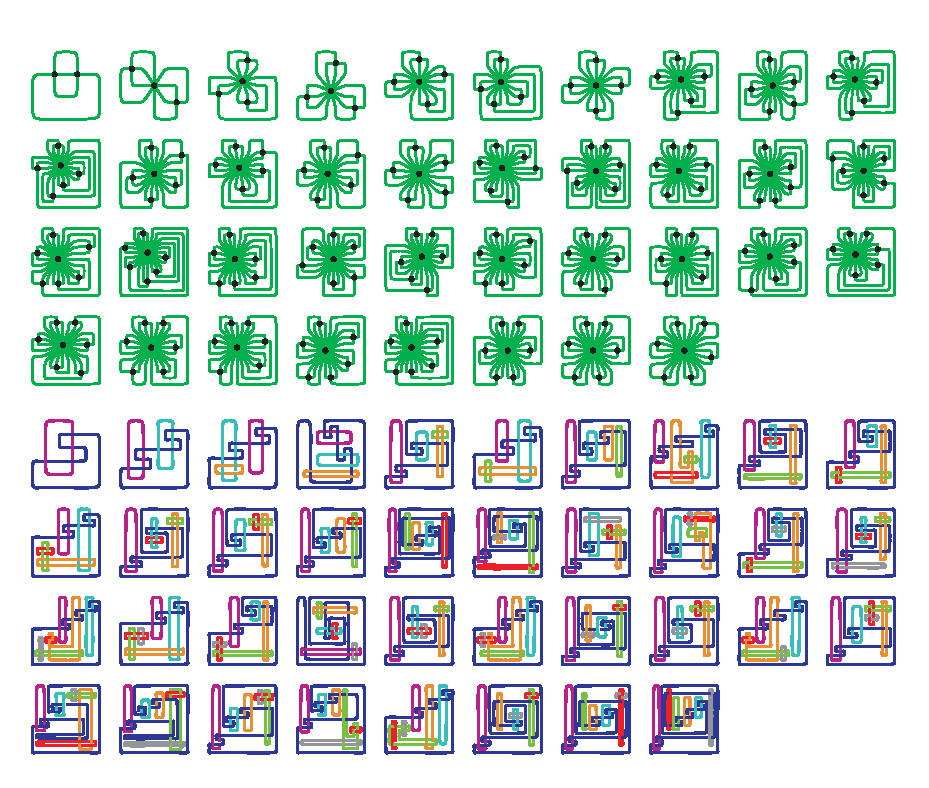
\psfig{file=fig/blinkLanguageExample.eps}
   \end{center}
   \vspace{-0.7cm}
   \caption{Toroidal sums or g-blink merges up to six copies of the quaternionic space}
   \label{fig:blinkLanguageExample}
\end{figure}

\section{Two final remarks}

\enlargethispage{1cm}

First. Recently we have extended the $U$ set to blinks with up to 10
edges. The number of blinks was increased from 3437 to 17948. The
number of potentially prime classes increased from 487 to 1025. The
number of composite classes increased from 14 to 40. We did not
attempt the topological classification of the classes 10.\_\_ using
3-gems.

Second. We have a contract with World Scientific Publisher to write
a book to be co-authored by S. Lins based on the material of this
thesis. The tentative title of this book: {\it All Shapes of Spaces:
a Genealogy of Closed Oriented 3-Manifolds} and it should be
finished by the year 2008.
